\subsection{Introduction}
The main application of the project is an Android app built on Unity. This allows the creation of a VR environment with ease. The only problem that arises from this choice is that it isn't possible to retrieve the data from the biosensor and send them to the smartphone directly as Unity doesn't allow a direct communication. As shown in figure \ref{fig:communication} the information from the biosensor are read first by a Computer and then sent to a Firebase server that stores the values. This values are then read by the Android application using a HTTP request.
\begin{figure}[h]
	\centering
	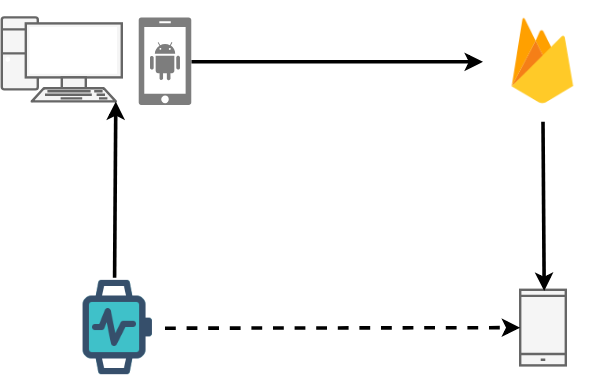
\includegraphics[scale=0.7]{ConnectionDiagram}
	\caption{Diagram that shows how the communication from the biosensor to the smartphone works.}\label{fig:communication}
\end{figure}

\subsection{Android Application}
Language used: C\#\\
Plugins:
\begin{itemize}
	\item ZXing
	\item Android Runtime Permissions
\end{itemize}

\subsection{Computer Client}
Language used: Java
Plugins:
\begin{itemize}
	\item ZXing
	\item JavaFX
\end{itemize}
